\documentclass{article}

\usepackage[top=2in, bottom=1.5in, left=1in, right=1in]{geometry}
\usepackage{fancyhdr} 		% page header
\usepackage{amsmath}
\usepackage{amssymb}
\usepackage{float}
\usepackage{graphicx}
\usepackage{url}
\usepackage{color}
\usepackage{tikz}
\usetikzlibrary{arrows,automata}
\usepackage{hyperref}

\pagestyle{fancy} 
\fancyhf{}
\fancyhead[L]{CS 540}
\fancyhead[R]{Fall 2017}

\def\x{\mathbf{x}}
\def\y{\mathbf{y}}
\def\w{\mathbf{w}}
\def\p{\mathbf{p}}

\begin{document}

\begin{center}
{\bf \large CS 540: Introduction to Artificial Intelligence

Homework Assignment \# 10

\vspace{0.5cm}

Assigned: 12/4 

Due: 12/15 before class} 
\end{center}

\vspace{1cm}

\begin{center}
{\bf \Large Hand in your homework:}
\end{center}

If a homework has programming questions, please hand in the Java program. 
If a homework has written questions, please hand in a PDF file.
Regardless, please zip all your files into hwX.zip where X is the homework number.
Go to UW Canvas, choose your CS540 course, choose Assignment, click on Homework X: this is where you submit your zip file. 

\vspace{1cm}

\begin{center}
{\bf \Large Late Policy:}
\end{center}

All assignments are due at the beginning of class on the due date. One (1) day late, defined as a 24-hour period from the deadline (weekday or weekend), will result in 10\% of the total points for the assignment deducted. So, for example, if a 100-point assignment is due on a Wednesday 9:30 a.m., and it is handed in between Wednesday 9:30 a.m. and Thursday 9:30 a.m., 10 points will be deducted. Two (2) days late, 25\% off; three (3) days late, 50\% off. No homework can be turned in more than three (3) days late. Written questions and program submission have the same deadline. 

Assignment grading questions must be raised with the instructor within one week after the assignment is returned.

\vspace{4pt}

\begin{center}
{\bf \Large Collaboration Policy:}
\end{center}

You are to complete this assignment individually. However, you are encouraged to discuss the general algorithms and ideas with classmates, TAs, and instructor in order to help you answer the questions. You are also welcome to give each other examples that are not on the assignment in order to demonstrate how to solve problems. But we require you to:
\begin{itemize}
\item not explicitly tell each other the answers
\item not to copy answers or code fragments from anyone or anywhere
\item not to allow your answers to be copied
\item not to get any code on the Web
\end{itemize}

In those cases where you work with one or more other people on the general discussion of the assignment and surrounding topics, we suggest that you 
specifically record on the assignment the names of the people you were in discussion with.

\newpage



\section*{Question 1: Neural Network [100 points, evenly among parts]}

We will build a neural network to perform binary classification.
Each input item has two real-valued features $x=(x_1, x_2)$, and the class label $y$ is either 0 or 1.
Our neural network has a very simple structure: 

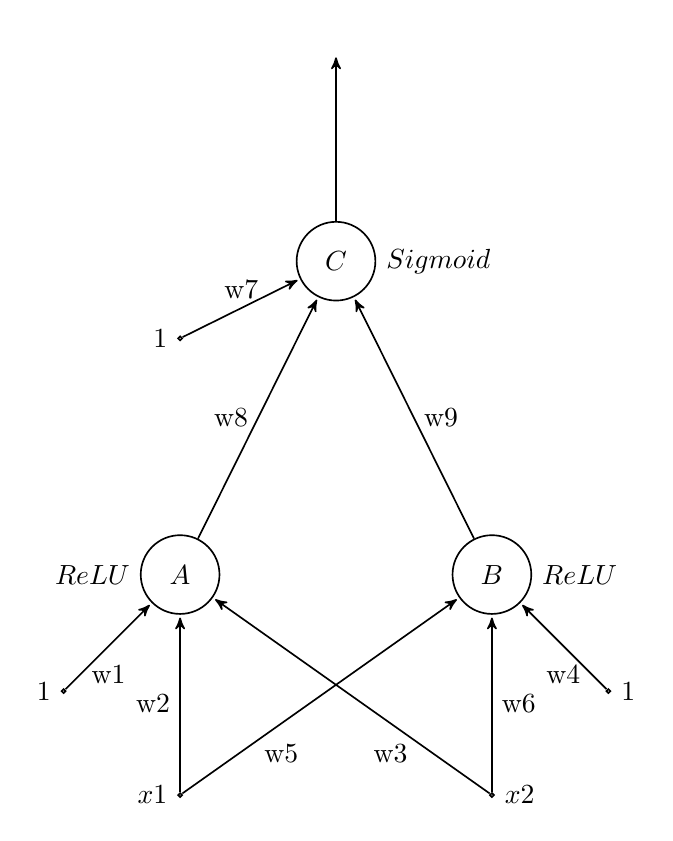
\begin{tikzpicture}[->,>=stealth',shorten >=1pt,auto,node distance=2.8cm,
                    semithick]
  \tikzstyle{state}=[circle,draw=black,text=black,minimum size=1cm]
  \tikzstyle{point}=[circle,draw=black,text=black,inner sep=0pt, minimum size=0.5mm]

  \node[state]         (A) [label=left:$ReLU$] {$A$};
  \node[state]         (C) [above right of=A, yshift=2cm, label=right:$Sigmoid$] {$C$};
  \node[state]         (B) [below right of=C, yshift=-2cm, label=right:$ReLU$] {$B$};
  \node[point]         (X1) [below of=A,label=left:$x1$] {};
  \node[point]         (X2) [below of=B,label=right:$x2$] {};
  \node[point]         (Y1) [below left of=A, xshift=0.5cm, yshift=0.5cm, label=left:$1$] {};
  \node[point]         (Y2) [below right of=B, xshift=-0.5cm, yshift=0.5cm, label=right:$1$] {};
  \node[point]         (Y3) [below left of=C, yshift=1cm, label=left:$1$] {};
  \node[circle]        (Z) [above of=C] {};




  \path (A) edge              node [left] {w8} (C)
        (B) edge              node [right] {w9} (C)
        (C) edge              node {} (Z)
        (X1) edge             node {w2} (A)
             edge             node [below, xshift=-0.5cm, yshift=-0.5cm] {w5} (B)
        (X2) edge             node [below, xshift=0.5cm, yshift=-0.5cm] {w3} (A)
             edge             node [right] {w6} (B)
        (Y1) edge             node [above, yshift=-6mm] {w1} (A)
        (Y2) edge             node [above, yshift=-6mm] {w4} (B)
        (Y3) edge             node [above] {w7} (C);
\end{tikzpicture}

There is one hidden layer with two hidden units A, B, and one output layer with a single output unit C.
The input layer is fully connected to the hidden layer, and the hidden layer is fully connected to the output layer.
Each unit also has a constant bias 1 input with the corresponding weight. See figure below.
Units A are B are ReLU, namely 
$$f_A(z)=f_B(z)=\max(z, 0).$$
Unit C is a sigmoid,
$$f_C(z)=\sigma(z)=\frac{1}{1+e^{-z}}.$$




Write a program \textbf{Neural.java} with the following command line format:
\begin{verbatim}
$java Neural FLAG [args]
\end{verbatim}
Where the optional arguments are real valued.


\begin{enumerate}
\item
This neural network is fully defined by the nine weights $w_1, \ldots, w_9$.
We will first focus on predictions \emph{given} fixed weights.

Remark: we will use both single index and double index to refer to a weight.
Single index corresponds to the figure above.
Double index, on the other hand, is used to describe the algorithm and denotes the ``from $\rightarrow$ to'' nodes that the edge is connecting.
For example, $w_8$ is the same as $w_{A,C}$, $w_2$ is the same as $w_{x_1, A}$, and $w_1$ is the same as $w_{1,A}$ where we used ``1'' to denote the constant bias input of one.
These should be clear from the context.

Recall in a neural network for any unit $j$, it first collects input from lower units:
$$u_j = \sum_{i: i\rightarrow j} w_{ij} v_i$$
where $v_i$ is the output of lower unit $i$. Specifically, if $i$ is an input unit then $v_i=x_i$; if $i$ is the bias then $v_i=1$.
The unit $j$ then passes $u_j$ through its nonlinear function $f_j()$ to produce its output $v_j$:
$$v_j = f_j(u_j).$$

When FLAG=100, arg1 ... arg9 are the weights $w_1, \ldots, w_9$, and arg10=$x_1$, arg11=$x_2$.
Print $u_A, v_A, u_B, v_B, u_C, v_C$ on the same line separated by space. When printing real values, show 5 digits after decimal point by rounding (but do not round the actual variables).
For example,
\begin{verbatim}
$java Neural 100 0.1 0.2 0.3 0.4 0.5 0.6 0.7 0.8 0.9 1 -1
0.00000 0.00000 0.30000 0.30000 0.97000 0.72512 

$java Neural 100 1 0.9 0.8 0.7 0.6 0.5 0.4 0.3 0.2 -0.2 1.7
2.18000 2.18000 1.43000 1.43000 1.34000 0.79249 

$java Neural 100 4 3 2 1 0 -1 -2 -3 -4 -4 1
-6.00000 0.00000 0.00000 0.00000 -2.00000 0.11920 
\end{verbatim}

\item
Given a training item $x=(x_1, x_2)$ and its label $y$, the error made by the neural network on the item is defined as
$$E = \frac{1}{2}(v_C - y)^2.$$
The partial derivative with respect to the output layer variable $v_C$ is 
$$\frac{\partial E}{\partial v_C} = v_C - y.$$
The partial derivative with respect to the intermediate variable $u_C$ is 
$$\frac{\partial E}{\partial u_C} = \frac{\partial E}{\partial v_C} f_C'(u_C).$$
Recall $f_C'(u_C) = \sigma'(u_C) = \sigma(u_C)(1-\sigma(u_C)) = v_C (1-v_C)$.

When FLAG=200, arg1 ... arg9 are the weights $w_1, \ldots, w_9$, arg10=$x_1$, arg11=$x_2$, and arg12=$y$.
Print $E$, $\frac{\partial E}{\partial v_C}$, and $\frac{\partial E}{\partial u_C}$ on the same line separated by space. 
For example,
\begin{verbatim}
$java Neural 200 0.1 0.2 0.3 0.4 0.5 0.6 0.7 0.8 0.9 1 -1 1
0.03778 -0.27488 -0.05479

$java Neural 200 1 0.9 0.8 0.7 0.6 0.5 0.4 0.3 0.2 -0.2 1.7 0
0.31402 0.79249 0.13032

$java Neural 200 4 3 2 1 0 -1 -2 -3 -4 -4 1 0
0.00710 0.11920 0.01252
\end{verbatim}

\item 
The partial derivative with respect to hidden layer variable $v_j$ is
$$\frac{\partial E}{\partial v_j} = \sum_{k: j\rightarrow k} w_{jk} \frac{\partial E}{\partial u_k}.$$
And 
$$\frac{\partial E}{\partial u_j} = \frac{\partial E}{\partial v_j} \frac{\partial v_j}{\partial u_j}.$$
Recall our hidden layer units are ReLU, for which
$$\frac{\partial v_j}{\partial u_j}=\frac{\partial \max(u_j, 0)}{\partial u_j}=\left\{
\begin{array}{ll}
1, & u_j \ge 0 \\
0, & u_j < 0 
\end{array}
\right.$$
Note we define the derivative to be 1 when $u_j=0$.

When FLAG=300, arg1 ... arg9 are the weights $w_1, \ldots, w_9$, arg10=$x_1$, arg11=$x_2$, and arg12=$y$.
Print $\frac{\partial E}{\partial v_A}$, $\frac{\partial E}{\partial u_A}$, $\frac{\partial E}{\partial v_B}$, and $\frac{\partial E}{\partial u_B}$
on the same line separated by space. 

\begin{verbatim}
$java Neural 300 0.1 0.2 0.3 0.4 0.5 0.6 0.7 0.8 0.9 1 -1 1
-0.04383 -0.04383 -0.04931 -0.04931

$java Neural 300 1 0.9 0.8 0.7 0.6 0.5 0.4 0.3 0.2 -0.2 1.7 0
0.03910 0.03910 0.02606 0.02606

$java Neural 300 4 3 2 1 0 -1 -2 -3 -4 -4 1 0
-0.03755 0.00000 -0.05006 -0.05006
\end{verbatim}

\item
Now we can compute the partial derivative with respect to the edge weights:
$$\frac{\partial E}{\partial w_{ij}} = v_i \frac{\partial E}{\partial u_j}.$$
When FLAG=400, arg1 ... arg9 are the weights $w_1, \ldots, w_9$, arg10=$x_1$, arg11=$x_2$, and arg12=$y$.
Print $\frac{\partial E}{\partial w_1}, \ldots \frac{\partial E}{\partial w_9}$ 
on the same line separated by space. 
For example,
\begin{verbatim}
$java Neural 400 0.1 0.2 0.3 0.4 0.5 0.6 0.7 0.8 0.9 1 -1 1
-0.04383 -0.04383 0.04383 -0.04931 -0.04931 0.04931 -0.05479 0.00000 -0.01644

$java Neural 400 1 0.9 0.8 0.7 0.6 0.5 0.4 0.3 0.2 -0.2 1.7 0
0.03910 -0.00782 0.06647 0.02606 -0.00521 0.04431 0.13032 0.28411 0.18636

$java Neural 400 4 3 2 1 0 -1 -2 -3 -4 -4 1 0
0.00000 0.00000 0.00000 -0.05006 0.20025 -0.05006 0.01252 0.00000 0.00000
\end{verbatim}

\item
Now we perform one step of stochastic gradient descent.  With step size $\eta$, we update the weights:
$$w_i = w_i - \eta \frac{\partial E}{\partial w_i}, \;\; i=1\ldots 9.$$
When FLAG=500, arg1 ... arg9 are the weights $w_1, \ldots, w_9$, arg10=$x_1$, arg11=$x_2$, arg12=$y$, and arg13=$\eta$.
Print four lines:
\begin{enumerate}
\item the old $w_1 \ldots w_9$
\item the error $E$ under the old $w$
\item the updated $w_1 \ldots w_9$
\item the error $E$ after the update
\end{enumerate}
For example,
\begin{verbatim}
$java Neural 500 0.1 0.2 0.3 0.4 0.5 0.6 0.7 0.8 0.9 1 -1 1 0.1
0.10000 0.20000 0.30000 0.40000 0.50000 0.60000 0.70000 0.80000 0.90000
0.03778
0.10438 0.20438 0.29562 0.40493 0.50493 0.59507 0.70548 0.80000 0.90164
0.03617

$java Neural 500 1 0.9 0.8 0.7 0.6 0.5 0.4 0.3 0.2 -0.2 1.7 0 0.1
1.00000 0.90000 0.80000 0.70000 0.60000 0.50000 0.40000 0.30000 0.20000
0.31402
0.99609 0.90078 0.79335 0.69739 0.60052 0.49557 0.38697 0.27159 0.18136
0.29972

$java Neural 500 4 3 2 1 0 -1 -2 -3 -4 -4 1 0 0.1
4.00000 3.00000 2.00000 1.00000 0.00000 -1.00000 -2.00000 -3.00000 -4.00000
0.00710
4.00000 3.00000 2.00000 1.00501 -0.02002 -0.99499 -2.00125 -3.00000 -4.00000
0.00371
\end{verbatim}

\item
Long long ago, in a galaxy far far away, 117 students took an AI class.
We have a data set where $x_1$ is each student's score on homework 2, $x_2$ is their midterm score (both scaled to between 0 and 1), and the binary label $y$ is whether they received an A at the end of semester ($y=1$) or not ($y=0$).
We already randomly split the data set into a training set of $n=67$ items, an evaluation set with 25 items, and a test set with 25 items.  These files are denoted by the file names.
We will train the neural network to predict if a student will receive an A at the end of semester.

We first define one ``epoch'' as going over the training items once in the natural order:
\begin{enumerate}
\item FOR $j=1$ TO $n$
\item ~~~ $w_i = w_i - \eta \frac{\partial E_j}{\partial w_i}, \;\; i=1\ldots 9$
\item ~~~ PRINT $w$'s evaluation set error
\item END
\end{enumerate}
where $E_j$ is the error on the $j$-th training item.
In other words, this is stochastic gradient descent (except that we go over training items in order rather than randomly, but we shall ignore the difference for now).
Step (c) computes the evaluation set error as follows:
$$\sum_{k=1}^{25} \frac{1}{2}(v_C(x_k,w) - y_k)^2$$
where $(x_k, y_k)$ is an evaluation set item, and we used the notation $v_C(x_k,w)$ to mean the neural network output when the input is $x_k$ and the weights are $w$.

When FLAG=600, arg1 ... arg9 are the initial weights $w_1, \ldots, w_9$, arg10=$\eta$.
Run one epoch (i.e. going over the 67 training items once).
For each training item, print three lines:
\begin{enumerate}
\item $x_1, x_2, y$
\item the updated $w_1 \ldots w_9$
\item the evaluation set error under the updated $w$
\end{enumerate}
Therefore, you will print $67*3=201$ lines in total.
For example,
\begin{verbatim}
$java Neural 600 0.1 0.2 0.3 0.4 0.5 0.6 0.7 0.8 0.9 0.1
0.98000 0.87000 1.00000
0.10049 0.20048 0.30043 0.40055 0.50054 0.60048 0.70062 0.80034 0.90087
7.18915
0.92000 0.88000 0.00000
0.09486 0.19530 0.29548 0.39422 0.49471 0.59491 0.69358 0.79648 0.89110
7.12401
...
0.81000 0.75000 0.00000
-0.13841 0.01138 0.16820 0.06903 0.24590 0.41273 0.22295 0.73651 0.52301
3.93300
0.94000 0.69000 0.00000
-0.13841 0.01138 0.16820 0.06135 0.23868 0.40744 0.20827 0.73651 0.51442
3.87761
\end{verbatim}

\item
We now run $T$ epochs.  For clarity, we will only print evaluation set error at the end of each epoch.
When FLAG=700, arg1 ... arg9 are the initial weights $w_1, \ldots, w_9$, arg10=$\eta$, arg11=$T$.
At the end of each epoch, print $w$, then on a separate line the evaluation set error.
\begin{verbatim}
$java Neural 700 0.1 0.2 0.3 0.4 0.5 0.6 0.7 0.8 0.9 0.1 3
-0.13841 0.01138 0.16820 0.06135 0.23868 0.40744 0.20827 0.73651 0.51442
3.87761
-0.15422 0.01050 0.18620 -0.10760 0.12065 0.33611 -0.14930 0.73903 0.41698
2.99174
-0.18275 0.01188 0.22380 -0.19706 0.06861 0.31792 -0.35328 0.74892 0.41936
2.71163
\end{verbatim}

\item
FLAG=800 has the same input as FLAG=700.
But we will stop as soon as evaluation set error starts to increase after completing a whole epoch.
If evaluation set error decreases or stays the same, we will step after $T$ epochs.
Print the number of epochs that actually happened, the final $w$, and the evaluation set error on different lines.
Now you have a well-trained neural network.
For a test item $x$, you can make a binary classification prediction by thresholding the network output at 1/2 (predict positive class if the output is exactly 1/2).
Compute the test set classification accuracy (note: not the squared error) and print it, too.
\begin{verbatim}
$java Neural 800 0.1 0.2 0.3 0.4 0.5 0.6 0.7 0.8 0.9 0.1 10000
788
-3.51459 1.20379 4.45346 -2.72310 0.93258 3.44859 -3.99435 2.11219 1.63381
0.87178
0.96000

$java Neural 800 -0.8 0.5 0 -1 0 -0.7 -0.7 0.9 0.1 0.1 10000
2
-0.80000 0.50000 0.00000 -1.00000 0.00000 -0.70000 -0.65318 0.90000 0.10000
2.56847
0.72000
\end{verbatim}

\end{enumerate}
\end{document}
